\documentclass[conference]{IEEEtran}
\IEEEoverridecommandlockouts
% The preceding line is only needed to identify funding in the first footnote.
% If that is unneeded, please comment it out.
\usepackage{amsmath,amssymb,amsfonts}
\usepackage{algorithmic}
\usepackage{graphicx}
\usepackage{textcomp}
\usepackage{xcolor}
\usepackage{natbib}
\usepackage{graphicx}

\usepackage{todonotes}
\newcommand{\cit}[1][]{\todo[tickmarkheight=0.2cm]{cit #1}}

\def\BibTeX{{\rm B\kern-.05em{\sc i\kern-.025em b}\kern-.08em
    T\kern-.1667em\lower.7ex\hbox{E}\kern-.125emX}}
\begin{document}

% \title{Trading data biases for cognitive biases:\\some shortcomings of the XAI approach}

\title{Defining Explainability in the XAI field}

\author{\IEEEauthorblockN{Alvise de' Faveri Tron}
    \IEEEauthorblockA{\textit{Politecnico di Milano} \\
        alvise.defaveri@mail.polimi.it}}

\maketitle

\begin{abstract}
    \todo[inline]{TODO}
\end{abstract}

%-----------------------------------------------------------------%
\section{Introduction}
\label{sec:intro}

AI has become an increasingly mature technology nowadays, and it has gained an enormous traction especially in the last decade. Amazing results have been reached in this field, so much that some have described this phenomenon as the ``AI singularity'' \cit.

Many tasks that were exclusively carried out by humans in the past, for example
in the legal, law enforcement and medical fields, are now being considered
feasible for AI. \cit This poses a new series of challenges to our society,
which are destined to become more relevant as this technology becomes more
pervasive.

% by AI systems: some go as far as calling the current period a "fourth
% industrial revolution" \note{cit} caused by AI or talk about the "AI
% singularity" \note{cit} referring to the fact that nothing like this has been
% seen before in human history.

However, AI is far from being perfect: there
are still many shortcomings in current implementations of this technology.
AI systems tend to break in a sudden and unpredictable way, and the nature of many AI
algorithms is such that errors can be difficult to correct or even to identify, remaining undetected for potentially long periods. The problem of understanding AI is not just a usability problem involving the end users, but it also affects the developers of these systems, who are mostly blind
towards what they build: this is known as the ``black box'' problem in AI. \cit

Machine Learning and Neural Networks in particular, which are the most common
and performing AI techniques today, are difficult for humans to debug.
This poses huge ethical and practical concerns about whether we can trust this technology, especially since it is being employed for tasks that have complex, and sometimes unexpected, ethical consequences. \cit

Explainable Artificial Intelligence (XAI \cit) is a relatively new field of AI
that aims at addressing this problem. Many interesting results have been
achieved in this field, and many more are expected to come in the next years, but there
are still some fundamental problems that this approach seems to struggle with.

In particular, there seems to be a lack of uniform terminology across the
research community when it comes to XAI. There have been attempts to define the
notions of ``interpretability'', ``explainability'' along with
``reliability'',``trustworthiness'' and other similar notions, but there is no
general consensus on how to formally define and measure these properties.
\cit

In this paper we want to highlight how the lack of a formal definition of ``explainability" for XAI is not just due to a lack of standardization in this newborn field, but some aspects of this problem have their roots in profound questions about intelligence, thought and cognition, which are still mainly unsolved today. We will try to propose a conceptual framework to define ``explainability'', identifying some of the problem's dimensions, in order to analyze those aspects that are not related to a specific solution. We will highlight how the problem of measuring these dimensions is more than just a technical problem, and that the subjective nature of explainability can cause cognitive biases to be accentuated in the interpretation of an AI output.

In this context, we will use  the words “explainability” and “interpretability”
interchangeably, as suggested in \cit.

The reminder of this paper is organized as follows.

Section~\ref{sec:background} will provide  some examples that we consider relevant to understand
the XAI problem in detail.

In Section~\ref{sec:xai} we give a more specific definition of XAI and a general
overview of the solutions that are being developed in this framework.

Section~\ref{sec:explainability} tries to break down the concept of explainability in several dimensions, which can be used to identify and classify AI explanations.

Finally, in Section~\ref{sec:missing} we highlight the connection between these aspects and some external problems that prevent us from being able to give a precise definition of ``explainability'' for AI, in particular the difference between causality and correlation and the problem of defining intentionality and intelligence for machines.

%-----------------------------------------------------------------%
\section{Background}
\label{sec:background}

% \subsection{Machine Learning} \label{sec:ml}

% One very popular and effective technique in AI is Machine Learning, and in
% particular Supervised Learning \cit. This approach generally consists in
% \textit{training} an algorithm by giving it as input a large number of
% instances of a given problem and letting it figure out on its own the best way
% to model it. The strength of this technique is that no previous knowledge of
% the model of the problem is needed, nor it can be enforced generally, and this
% is exactly where this technology gets an edge over more traditional computer
% science approaches.

% \todo[inline]{rimuovere?}

% \subsection{Artificial Neural Networks} \label{sec:nn}

% A particular way of implementing a Machine Learning algorithm is through
% Artificial Neural Networks (ANN), which are an extremely powerful tool that is
% being employed for many complex problems nowadays, from computer vision to
% data analysis, showing unprecedented results. The idea is to have a fixed
% structure made of interconnected \textit{neurons}, whose connections, called
% \textit{weights}, are modified in the learning phase by the learning
% algorithm.

% \todo[inline]{rimuovere?}

\subsection{AI in practice}
\label{sec:aiprog}

The word ``Artificial Intelligence'' has historically been used with many meanings, even more so today that this subject is receiving a lot of media attention, and the term is being used loosely to indicate a very large and varied set of technologies. Without trying to define the concept of Artificial Intelligence as a whole, which is per-se a matter of debate \cit, we will try to give some distinctive traits of what is commonly refer to as ``AI'' in the modern Computer Science field.

For the purpose of this paper, we can define AI as a set of \textit{meta-}algorithms used to explore the solution space of problems that are generally vast and complex, i.e. for which there is no simple a-priori rule that tells us where the (best) solution is.

Let's take for example the problem of recognizing whether an image contains a dog or a cat. The problem is trivial if we want to match the exact image of a specific dog, but it becomes overwhelmingly difficult if we want to construct a set of rules that define what is the shape of a \textit{generic} dog in terms of pixel patterns. Humans have generally no problem at identifying a dog in a photograph even if it's the first time they see it, yet we are not able to express exactly the set of rules that we applied to recognize the ``dogness'' characteristic in that set of pixels.

This is an example of a problem with a vast solution space (the number of patterns that can be recognized in an image of a given size) and no a-priori rule to know which is the best. The fact that the solution space is huge means we cannot think of exploring it exhaustively, so we need an ``intelligent'' way to explore it. This is what AI is about.

One particular aspect that can be found in many of today's top-performing technologies, such as Neural Network, Ant Colony Optimization, Genetic Algorithms etc. is that they are not deterministic: there is no guarantee of finding the best solution in the solution space, nor that the same algorithm will find the same solution if the initial conditions are different. Introducing some kind of randomness has in many cases provided a huge benefit, and since for many complex problems even a best-effort solution is acceptable, this approach has thrived.

A particularly effective technique is Machine Learning, which generally consists in
\textit{training} an algorithm by giving it as input a large number of
instances of a given problem and letting it figure out on its own the best way
to model it. The strength of this technique is that no previous knowledge of
the model of the problem is needed, nor it can be enforced generally, and this
is exactly where this technology gets an edge over more traditional computer
science approaches.

When implementing the aforementioned techniques, the programmer gets to decide
only some of the aspects of the implementation, e.g. the number of layers, neurons and
activation functions in the case of Neural Networks, but is not in control of
the whole output of the algorithm, which is \textit{learned} using the data it
is fed with. While this is immensely powerful, it is also very problematic from
the point of view of the developer, which is by design unable to specify all the behavior of the algorithm.
% %-----------------------------------------------------------------%
% \section{The Problem} \label{sec:problem}

\subsection{AI failures}
\label{sec:aifails}

The observation of how AI systems behave in the real world has shown us one
interesting fact: when these systems break, they tend to break hard. A single
misprediction made by an AI system can cast a
shade on the correctness of the whole model itself, on the data it has been
trained on or on its design. There's rarely such thing as ``fixing one line of
code" on deep neural networks that have been trained on millions of data points:
once its trained, you either add more data or start again from scratch, which
can be a very high price to pay in terms of time and computational power.

\todo[inline]{Esempi concreti invece che claim astratti?}

Moreover, these kind of errors are generally difficult to predict in advance: an
AI algorithm can perform very well on a high number of inputs, but have a weak
point that is only discovered way after the AI has been deployed. The same
people that design and train the algorithm have generally little knowledge about
what model the network is going to produce at the end, and when it does the only
way of verifying its correctness is black box testing, for which the input space
is generally huge.

All these considerations have encouraged the AI industry and the governments to
tackle the problem of understanding an AI model and "opening" the black box.

\subsection{A toy example}
\label{sec:example}

As an example of the problem of explaining an AI system, a representation of a
Neural Network's conceptual structure is depicted in Figure~\ref{fig:nn}.

\begin{figure}[ht!] \centering 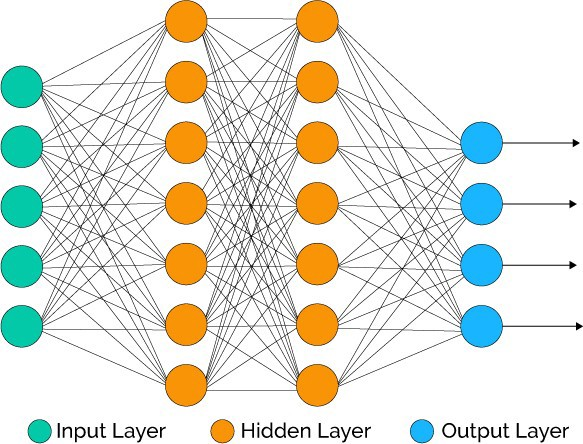
\includegraphics[width=0.8 \linewidth]{images/nn}
    \caption{Simple representation of an Artificial Neural Network}
    \label{fig:nn} \end{figure}

The graphical representation is useful for understanding the general
architecture of a Neural Network, but it doesn't really tell us anything about
how the Neural Network actually works, i.e. what is the relationship between a
certain input and a certain output.

We could give a more precise representation of this dependency in
Figure~\ref{fig:mathnn}, which explicitly defines the mathematical relationship
between the input and the output. Without going into the details of the
mathematical formula, we can see how we would still have a hard time
understanding what a Neural Network does if we were to adopt this
representation.

\begin{figure}[ht!] \centering
    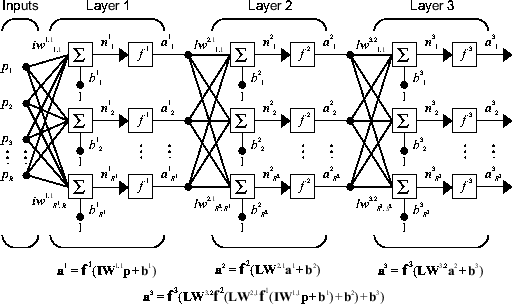
\includegraphics[width=0.9\linewidth]{images/nmodel} \caption{Mathematical
        equivalent representation} \label{fig:mathnn} \end{figure}

On the other hand, Figure~\ref{fig:dectree} represents a \textit{Decision Tree},
another family of AI algorithms. While on one hand we can easily agree that this
type of representation is more intelligible and tells us more about how the AI
algorithm constructed its model, we have to deal with the fact that Neural
Networks generally perform better than Decision Trees.

\begin{figure}[ht!] \centering
    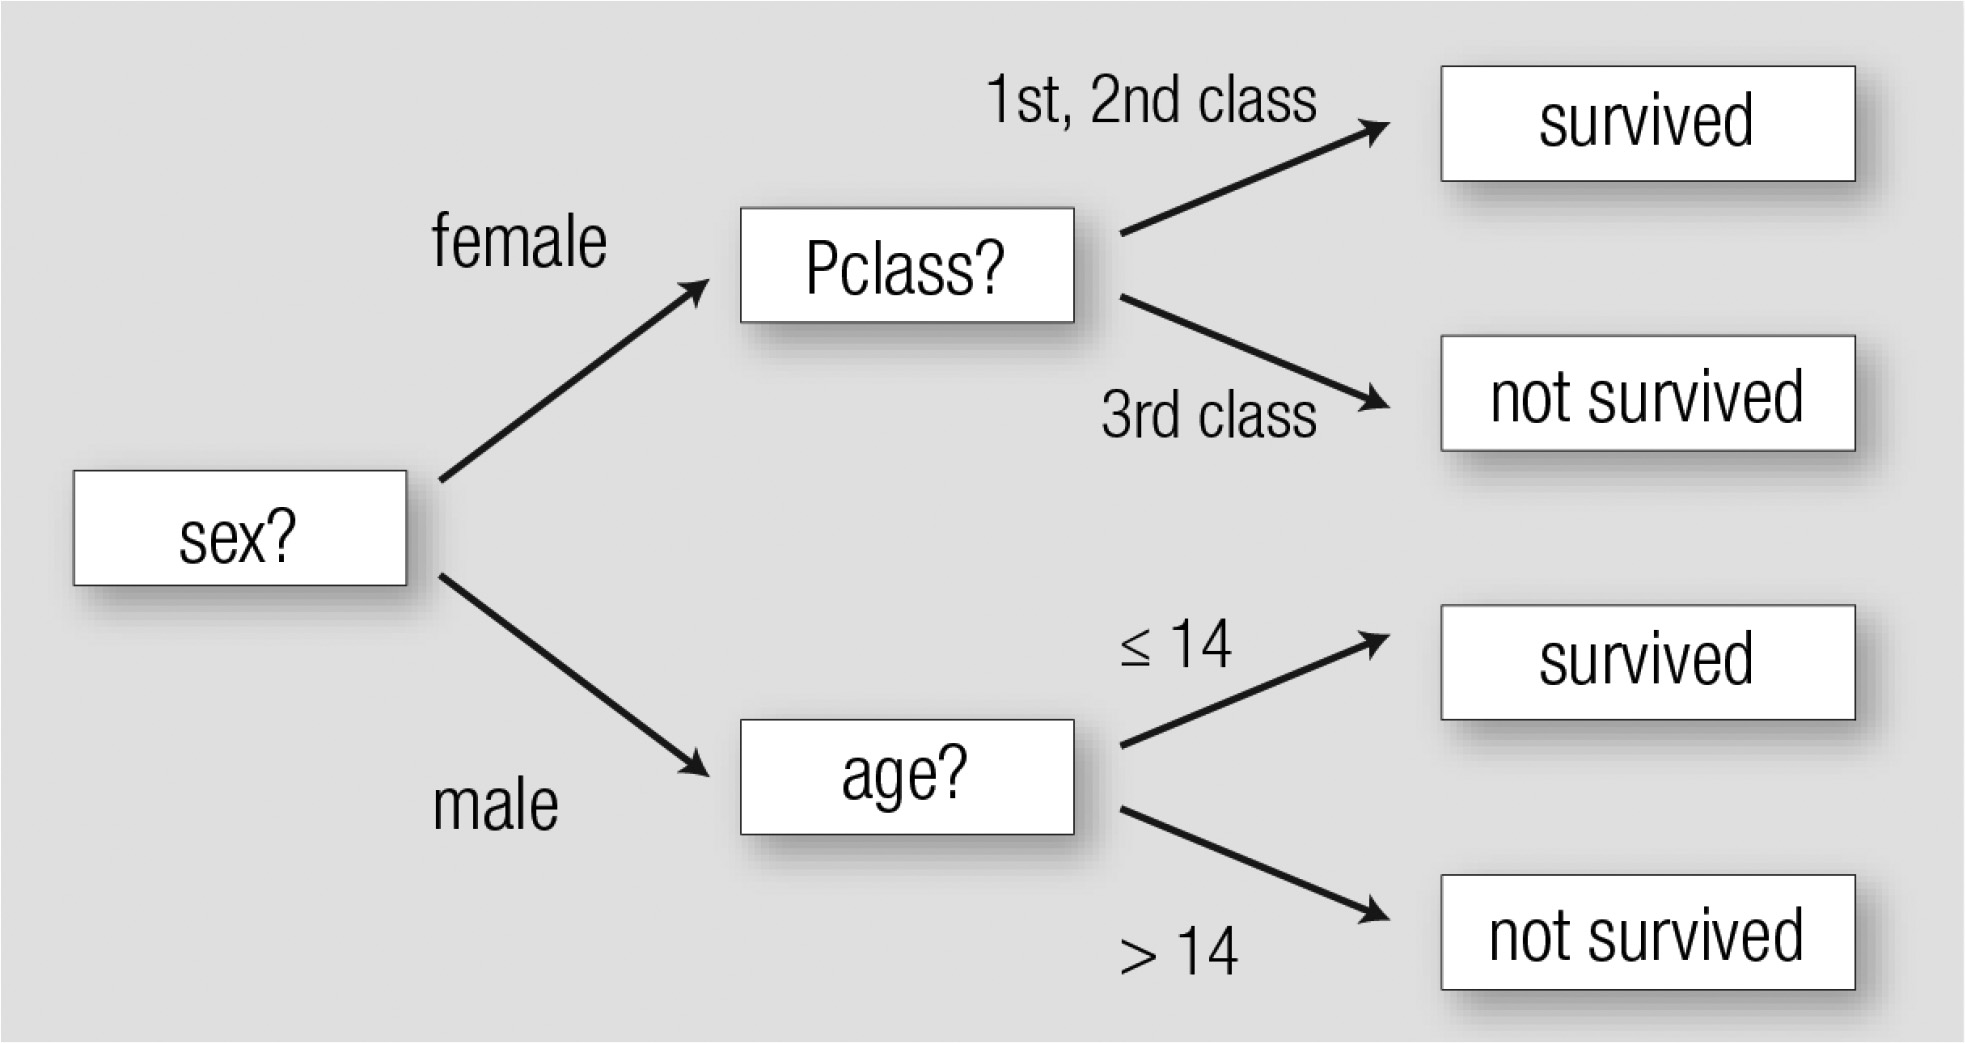
\includegraphics[width=0.9\linewidth]{images/dectree} \caption{A simple
        Decision Tree} \label{fig:dectree} \end{figure}

This simple example shows how the solution space to the explainability problem
has multiple dimensions, constraints and trade-offs that have to be taken into
account.

%-----------------------------------------------------------------%
\section{The XAI approach}
\label{sec:xai}

\subsection{The goal}

Explainable AI is a concept that was recently formalized in a call for papers
\todo[inline, inlinewidth=1.5cm, noinlinepar]{rephrase} made by DARPA \cit, the
same agency where the word "Artificial Intelligence" was born in the first place
\cit. It is meant to be describe a new set of Artificial Intelligence systems
which are designed to be easier to understand by humans. In particular, the
goals of XAI is making artificial intelligence more:

\begin{itemize}
    \item \textbf{Easy to debug} and correct
    \item \textbf{Predictable}, so that companies and governments adopting this
          technology can be aware of the possible weaknesses of a their models,
          and can be held responsible when using bad algorithms
    \item \textbf{Trustful} for operators and end-users of this technology
\end{itemize}

Figure~\ref{fig:xai} is taken from the DARPA presentation on XAI and describes
the kind of goals for which it has been proposed.


\begin{figure}[h!] 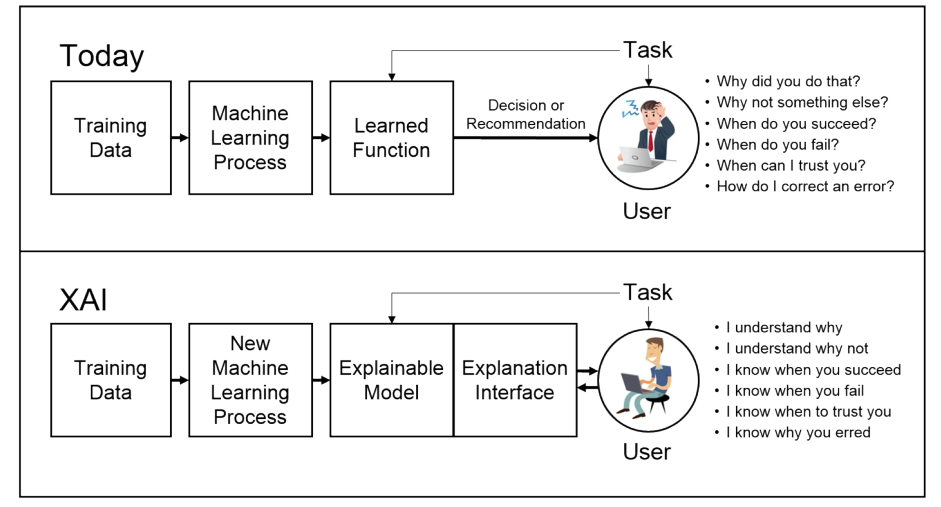
\includegraphics[width=\linewidth]{images/xai.png}
    \caption{The XAI concept \todo[inline]{cit} } \label{fig:xai} \end{figure}

The creation of XAI requires the join effort in a variety of research fields,
from Computer Science to Cognitive Psychology, and there is still a lot of work
to do. Nevertheless already many papers have been submitted on the subject \cit,
indicating a growing interest of the research community towards this subject.

\subsection{Current Solutions}
\label{sec:solutions}

Given the highly experimental nature of this topic, many different solutions
have been proposed by various papers in the framework of XAI, which vary greatly
in intended use, goal and adopted approach. Giannotti et al. \cit contains an exhaustive classification of the existing XAI
solutions and their respective strengths and weaknesses. With no aim of being
comprehensive or in any way technically precise, here we give a more abstract
classification of popular XAI solutions, based their general approach to the
problem.

XAI approaches might be classified as:

\begin{enumerate}
    \item \textbf{Visualization}: improving the understanding of a model using a
          better way to visualize its internals. One popular application of this
          approach is computer vision, where features of the learned model might
          be mapped onto the input image. \cit
    \item \textbf{Simplification}: similarly to the idea explained in
          Section~\ref{sec:example}, this approach consists in trying to adopt
          simpler models or simplify already existing models to just a set of
          important features. \cit
    \item \textbf{Approximation}: once a model has been produced by an AI, one
          explanation technique is to try and understand the dependencies
          between inputs and outputs by trying to find which output change is
          triggered by a given input change. Most of the times this means, in
          practice, creating a behavioral model of the algorithm which is
          parallel to the algorithm itself, and has no immediate correlation
          with the algorithm's internal structure.
    \item \textbf{Explanation by Example}: a nice information to have when
          trying to understand an AI model, especially in the case of
          classifiers, is an example, or a \textit{prototype}, of how the AI
          thinks that a typical member of a given class should appear. This can
          be realized in many ways, for example by attaching to a classification
          output a set of minimal changes to the input that would cause the
          output to be modified, or specify a partially filled object for each
          class.
\end{enumerate}

\todo[inline]{Immagini esemplificative}

\todo[inline]{Si può integrare con una classificazione più classica delle tecniche (internal vs external ecc)}



%-----------------------------------------------------------------%
\section{Defining Explainability}
\label{sec:explainability}

As we anticipated in Section~\ref{sec:intro}, one fundamental problem in
the field of XAI is that there is no single conventional notion of
explainability.

If, on one hand, many solutions have already been proposed to tackle the
problem, with various claims regarding their interpretability, on the other hand
the lack of a formal definition seriously challenges the findings of these
researches, casting a shade of doubt on the proposed solutions.

Mythos\cit goes as far as considering the term itself ill-defined, therefore
stating that claims about interpretability generally have a quasi-scientific
nature. Giannotti\cit on the other hand, in a review of the current state of the
art, considers the lack of a mathematical description as an obstacle for the
future development of this field. The DARPA paper \cit itself defines the
formalization of an evaluation metric for explanations as one of the goals of
the XAI project, to be developed in parallel with technical solutions.

Without discouraging the research on this matter, we want to highlight that this
is easier said than done.

\subsection{What is the scope?}

Before evaluating an explanation interface or an XAI system in general, we
should ask ourselves at least the following questions:

\

\textbf{Explainable to whom?} The concept of \textit{user} of an AI system is
not always well defined, nor is the concept of user of an explanation. This
might include:

\begin{itemize}
    \item The \textbf{developer} of the AI system, as he is only partially in
          control of what the algorithm does (refer to Section~\ref{sec:aiprog})
    \item The \textbf{operator} of an AI system: many AI algorithms nowadays are
          being used as an input for a human to make decisions on a certain
          subject
    \item The \textbf{end user} which is affected by the decision of an AI
\end{itemize}

\

\textbf{Explainable for which purpose?} Different users have different needs,
that can partially overlap, when it comes to AI explanation. More in general,
whether a certain representation can be considered explanatory depends to some
degree on what it is being used for. In the case of XAI, some common purposes
are:

\begin{itemize}
    \item \textbf{Debugging}: finding errors or underperforming portions of the
          system
    \item \textbf{Human-in-the-loop}: creating systems where human and AI
          decisions can co-exist and influence each other
    \item \textbf{Validation}: understanding if a certain model is good enough
          to be deployed for a certain tasks, where it fails and what happens
          when it fails
    \item \textbf{Appeal AI decisions}: \footnote{This last goal is not
              explicitly listed in the original scope of XAI goals, but has
              gained traction recently with the publication of \textit{right for
                  an explanation} law in EU. \todo[inline]{cit}} giving the right to
          users and citizens that are affected by AI decisions to know,
          understand and possibly appeal decisions that are automated with
          AI systems
\end{itemize}

\

It appears quite evident that different XAI solutions with different scopes and
intended users cannot be compared in the same way.

\subsection{Possible Metrics}
\label{sec:dimensions}

Bearing in mind the different goals that an XAI system can have, we can identify
a series of characteristics that are different among different solutions:

\begin{itemize}
    \item \textbf{Complexity}: how many elements are there in the explanation?
    \item \textbf{Clearness}: how cognitively hard is the explanation? How
          difficult is it to understand the correspondence between the elements
          of the explanation and the information we are trying to gain?
    \item \textbf{Informativeness}: how much information, weighted on how
          meaningful is is, can be extracted by the explanation? E.g. does the
          explanation significantly modify the level of uncertainty about the AI
          behavior?
    \item \textbf{Fidelity}: how closely does the explanation represent the
          internal functioning of the system? Are all the facts inferred from
          the explanation also applicable to the original system?
\end{itemize}

Clearly, the choice of the evaluation metric

\subsection{Can we measure all of them?}

fidelity vs complexity

\subsection{Possible biases}

cognitive bias

%-----------------------------------------------------------------%
\section{Some fundamental issues}
\label{sec:missing}


\begin{itemize}
    \item causality vs correlation
    \item previous knowledge
    \item ethical implications
\end{itemize}

%-----------------------------------------------------------------%
\section{Conclusions}
\label{sec:conclusions}

In conclusion, the main problem of XAI is that there is no single definition of
what an explanation is, it depends on the purpose and on the user of the AI
system.

For this reason, these should be considered different problems, at least the
debugging problem vs the right of explanation problem: they are not correlated
and saying that one solves the other poses some threats on the quality of the
result itself.

``I always thought something was fundamentally wrong with the universe''

\citep{adams1995hitchhiker}

\bibliographystyle{plain}
\bibliography{references}
\end{document}
